%%____________________________________________________________________________||
\section{Aggregate search regions}
\label{sec:aggregate-signal-regions}

Inclusive searches for new physics typically use fine categorisation to allow
sensitivity to a wide range of models. However, this can make the use
of the search for re-interpretation impractical. 
This section describes how this categorisation may be simplified without neglecting the correlation 
between the search regions by defining aggregate search regions.

Considering the simplified likelihood defined in Equation~\ref{eq:full-likelihood},
the likelihood for aggregate search regions may be written by substituting the 
background predictions by,

\begin{align}
b_{i} + \theta_i \rightarrow b_I + \theta_I \equiv \sum_{i}b_{i} + \theta_I
\label{eq:b-agg}
\end{align}

where the sum is over all search regions being aggregated into search region $I$.
Note that the number of aggregate search regions must be fewer than the total number of search regions and 
every search region must be contained in a single aggregate search region. 
Similarly, the signal expectations and observed number of events are substituted by, 

\begin{align}
 s_{i}  \rightarrow s_{I} \equiv \sum_{i}s_{i},  &&  n_{i}  \rightarrow n_{I} \equiv \sum_{i}n_{i} 
\label{eq:b-agg}
\end{align}


The covariance matrix in the aggregate search regions is related to the full covariance matrix as, 

\begin{align}
V_{IJ}=\sum^N_{t=1}{\frac{(\sum_{i}b^t_i-b_{i})\times(\sum_{j}b^t_j-b_{j})}{N}} = \sum_{i}\sum_{j}V_{ij}
\label{eq:agg-cov}
\end{align}

where the sum is over all search regions being aggregated into search regions $I,J$.  The use of the simplified likelihood 
for the aggregated search regions relies on the same conditions outlined in Section~\ref{sec:simplified-likelihood}. 

\subsection{Example of the use of aggregate search regions}
\label{sec:agg-toy}

The same toy search described in Section~\ref{sec:sl-toy} is considered for use in an aggregated search. 
From Figure~\ref{fig:toy-example} it is clear that search regions 7 and 8  provide the dominant contribution to 
the sensitivity of the search as the ratio of the expected signal to the background is the largest in these two regions. 
One may therefore expect that search regions 1--6 can be neglected when deriving constraints on this particular BSM model. 
However, as the background expectations in these search regions are correlated with those in search regions 7 and 8, neglecting search regions 1--6 
will result in a loss of sensitivity.  
Alternatively, the search regions 1--6 may be aggregated using the covariance matrix shown in 
Figure~\ref{fig:covariance} and Equation~\ref{eq:agg-cov}. The resulting covariance
between the aggregate search regions is shown in Figure~\ref{fig:agg-covariance}.

\begin{figure}[hbt]
  \begin{center} 
   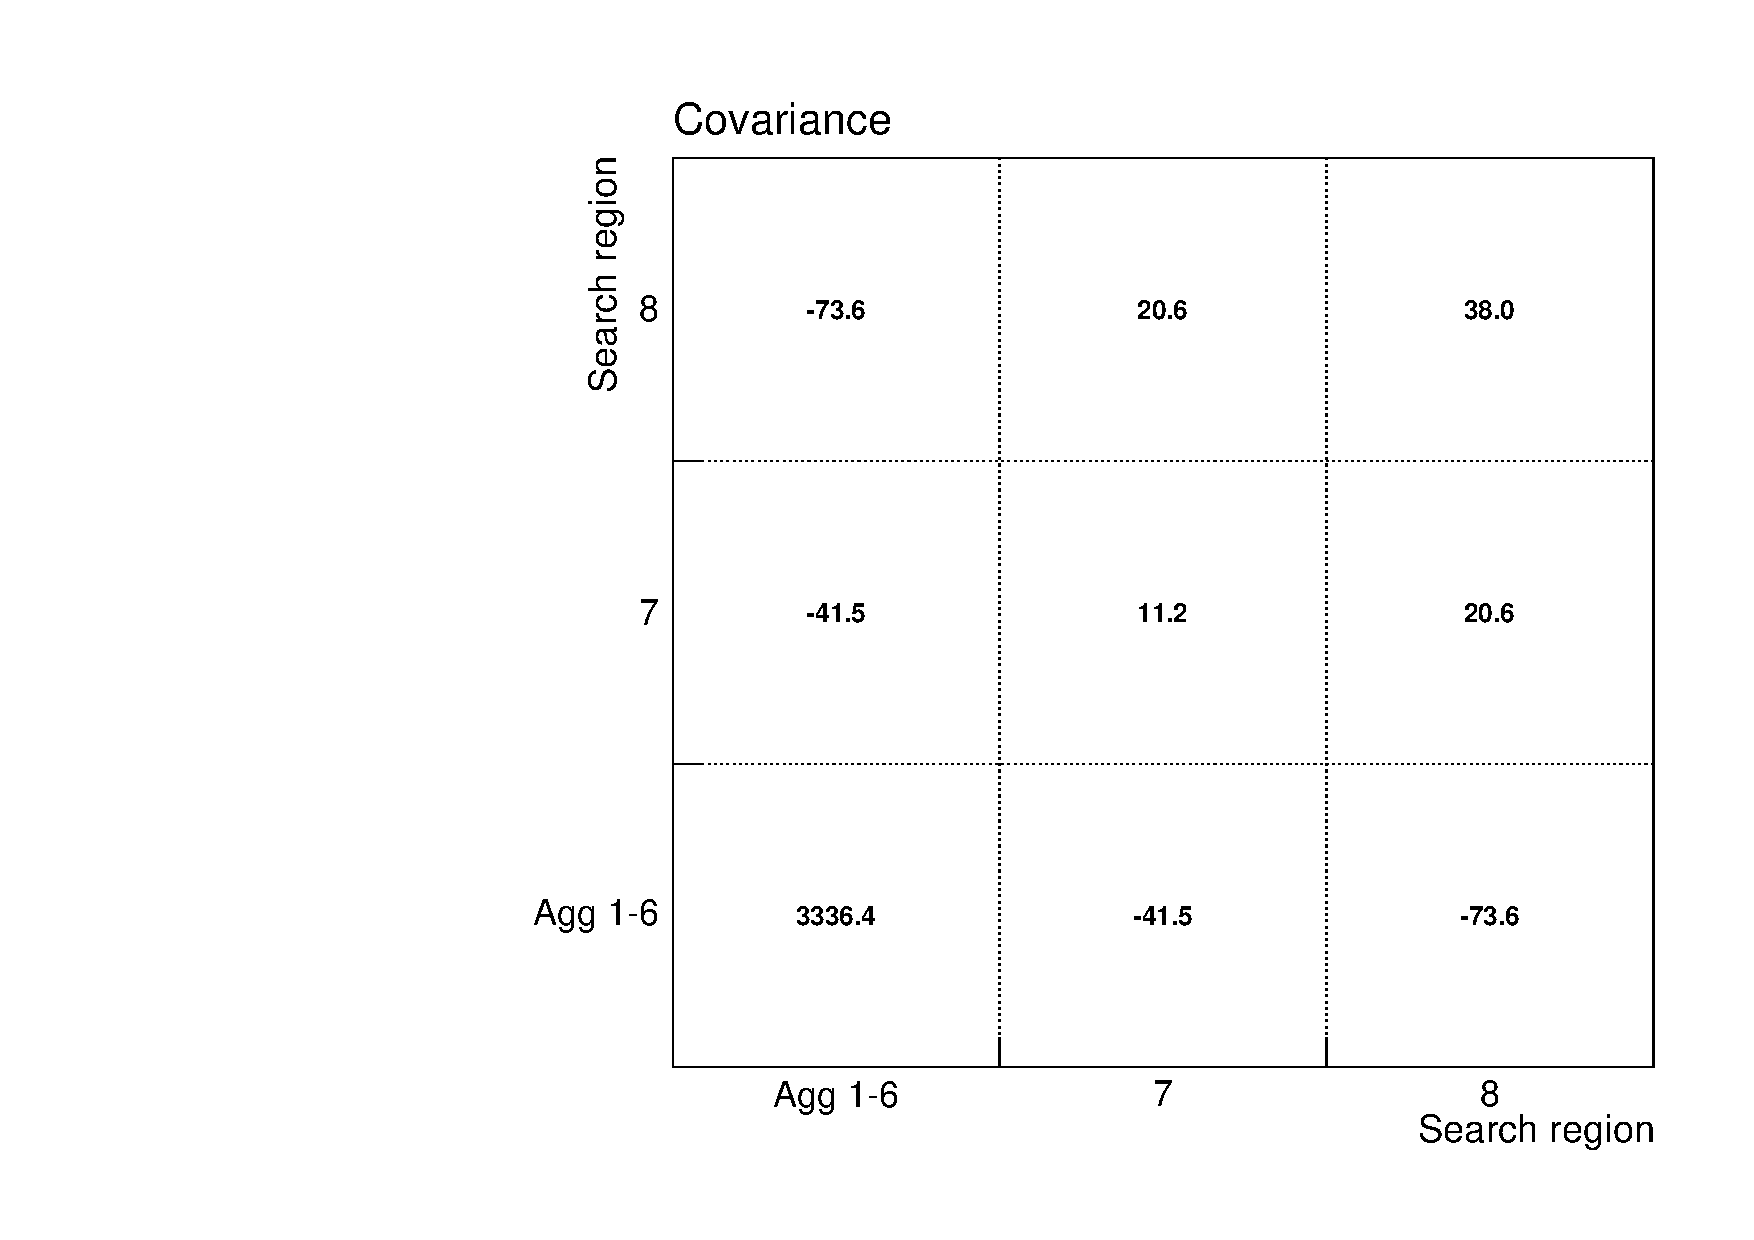
\includegraphics[width=1.5\cmsFigWidth]{figures/agg_htsearch_covariance.pdf}
   \caption{Covariance between the total rate of background contributions expected in each of the aggregated search regions}
   \label{fig:agg-covariance} 
  \end{center}
\end{figure}

Figure~\ref{fig:agg-likelihoodscan} shows the value of $q(\mu)$ as a function of $\mu$. The values when $q(\mu)$ 
is defined using the likelihood of Equation~\ref{eq:full-likelihood} using all 8 search regions, the aggregated search 
regions described above, and considering search regions 7 and 8 only are shown. There is good agreement between the curves using the 
aggregated search regions and using all 8 search regions. Neglecting the search regions 1--6 causes a change in the value
of $\hat{\mu}$. In addition, the width of the likelihood curve when neglecting these search regions is considerably
larger, implying a larger uncertainty estimate on $\mu$ and therefore poorer sensitivity to the BSM signal. 
This can be expected from the loss of constraint on the nuisance parameters when search regions 1--6 are neglected. 
Generically, the impact of removing search regions will depend on the size of the systematic uncertainties and their correlations 
between the search regions used and those which are neglected.

\begin{figure}[hbt]
  \begin{center} 
   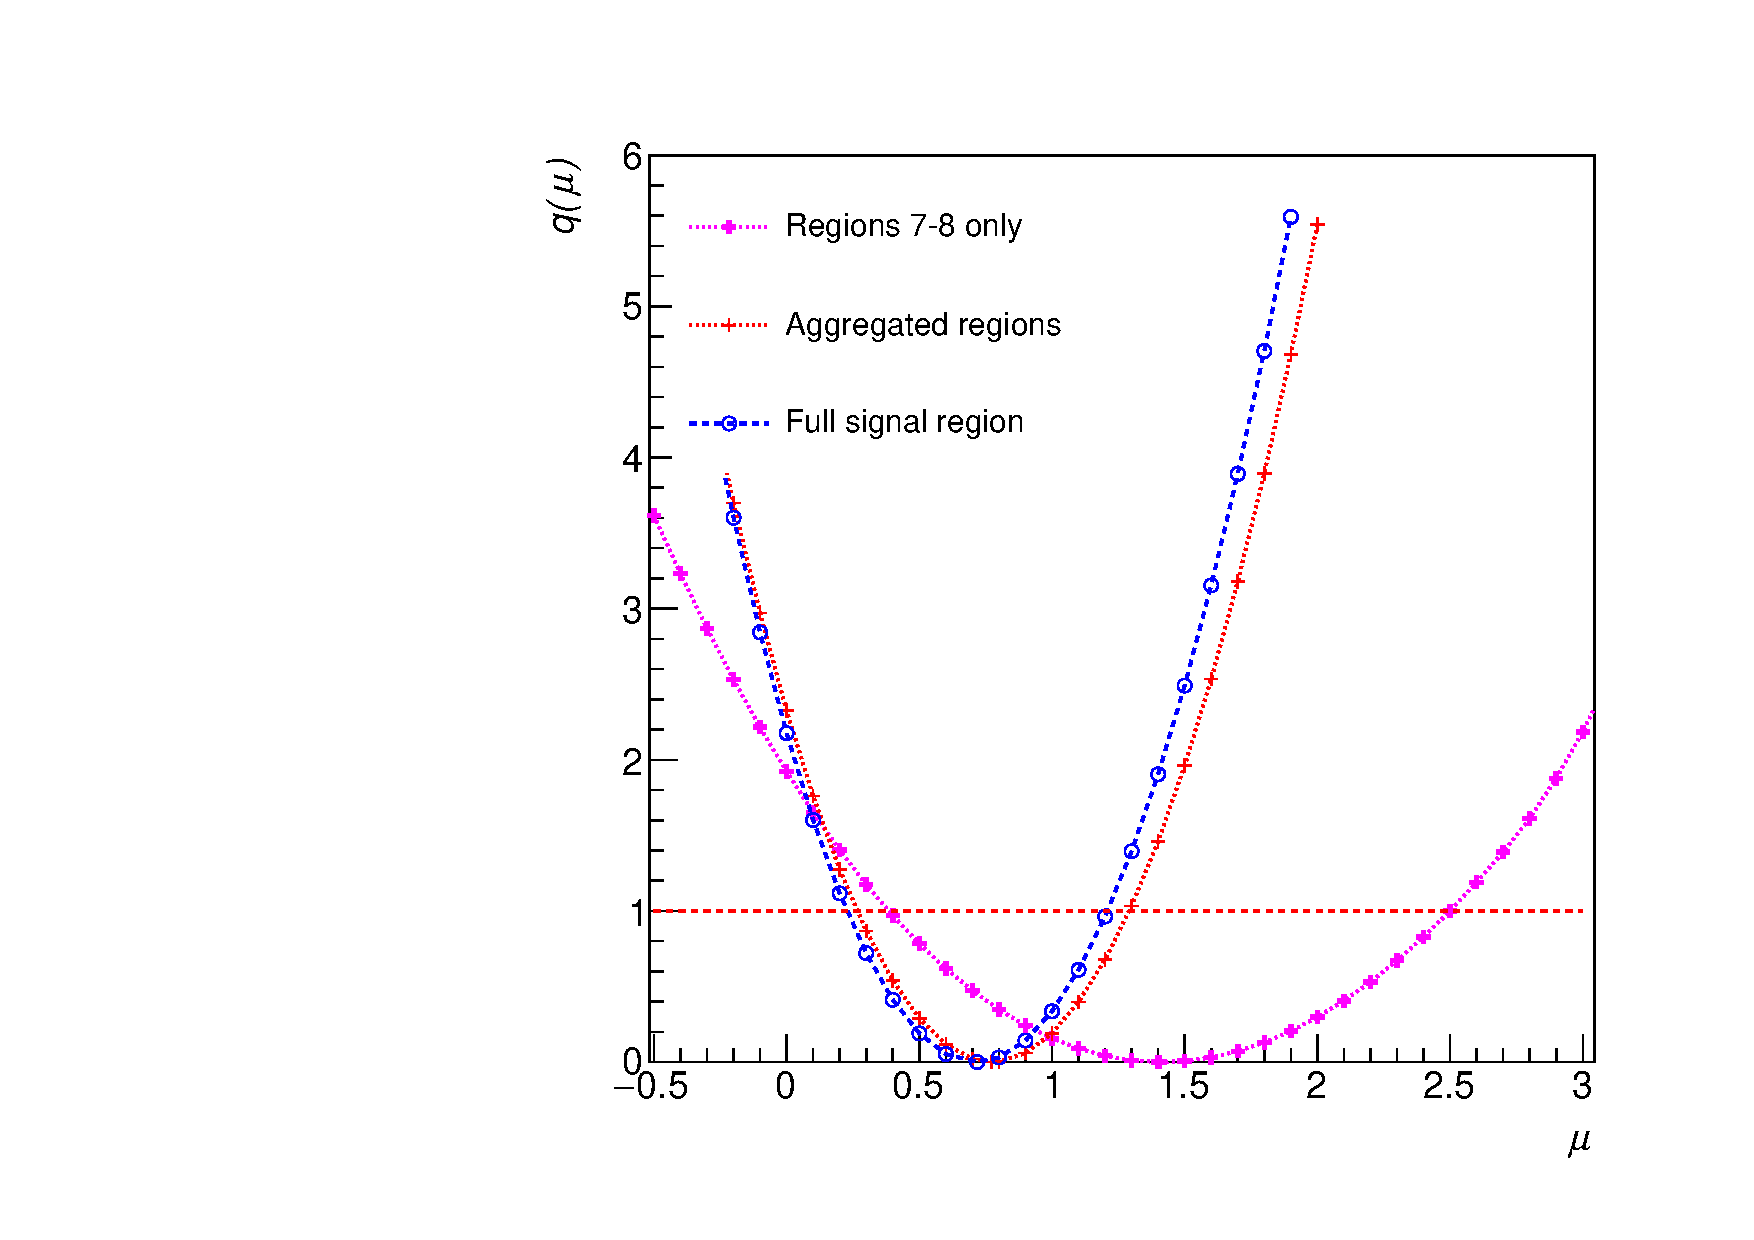
\includegraphics[width=1.5\cmsFigWidth]{figures/r_agg.pdf}
   \caption{The value of $q(\mu)$ defined using the simplified likelihood considering all 8 search regions (open blue points), the aggregated search regions (thin red crosses),
   and search regions 7 and 8 only (open magenta crosses).}
   \label{fig:agg-likelihoodscan} 
  \end{center}
\end{figure}
